\chapter{Panoramica generale sulle reti P2P}\label{panoramica-generale-sulle-reti-p2p}

Negli ultimi anni si è assistito ad una progressiva alterazione delle "leggi" che regolano il mondo dell'hardware informatico in campo consumer: l'aumento della potenza di calcolo del singolo elaboratore non è più economicamente conveniente\footnote{Come anche previsto da Moore: \url{https://it.wikipedia.org/wiki/Legge_di_Moore\#Seconda_legge_di_Moore}}.

Per fortuna la soluzione è stata immediata e consiste nello sfruttamento di più elaboratori collegati in rete che condividono (genericamente parlando) risorse. Sebbene per compiti specifici risulti spesso conveniente creare una rete ad-hoc, per l'utilizzo di tutti i giorni da parte dell'utente comune, la rete per eccellenza risulta essere senza ombra di dubbio la rete Internet. A causa di questa sua centralità, è stata scelta come base per lo sviluppo di applicazioni dedicate alla condivisione di risorse di vario tipo da parte di utenti con interessi in comune, creando di fatto una sottorete virtuale fondata sulla rete Internet.
%TODO sistemare sta frase scritta da cani

Questa convidisione di risorse da parte di utenti per un interesse comune definisce il nucleo di quelle che vengono chiamate \textbf{reti Peer-to-Peer}, da qui in avanti abbreviate come \emph{reti P2P}. Data la grande diffusione di queste reti e i loro svariati obiettivi, è comprensibile che ci siano molti disaccordi sulla definizione esatta di \emph{rete P2P}.

Una classificazione molto adatta agli scopi di questo documento è quella presente in \cite{core-concepts-p2p} che distingue tre diversi livelli di rete:

\begin{enumerate}
\def\labelenumi{\arabic{enumi}.}
\item
  \textbf{Infrastrutture P2P}, il cui scopo è porre le basi per i   livelli successivi fornendo funzioni di comunicazione, integrazione e   ``traduzione'' tra le varie componenti della rete. In particolare   forniscono servizi che permettono la localizzazione e la comunicazione   tra gli utenti (da ora in avanti \textbf{peer}) e l'identificazione,   l'utilizzo e lo scambio delle risorse, oltre che l'implementazione   delle politiche di sicurezza quali autenticazione e autorizzazione.
\item
  \textbf{Applicazioni P2P}, che utilizzano i servizi offerti dal   livello di infrastruttura per offrire all'utente (qui inteso come   essere umano interagente con la macchina, la quale è il peer vero e   proprio) le funzionalità della rete. Sono in pratica le interfacce tra   l'infrastruttura e la persona.
\item
  \textbf{Fenomeni sociali} derivanti dall'utilizzo delle applicazioni   P2P. Spesso infatti la forte coesione di intenti tra gli utenti di una   rete P2P porta alla nascita di comunità virtuali, centri di   aggregazione e correnti di pensiero che esulano dalla sfera   prettamente informatica.
\end{enumerate}

Come si vedrà più avanti nel corso della trattazione, la rete Bitcoin è caratterizzata da tutti e tre i livelli in modo molto più peculiare di altre reti P2P maggiormente diffuse e famose.

\section{Distribuzione dei file in una rete P2P}\label{distribuzione-dei-file-in-una-rete-p2p}

La risorsa indubbiamente più abbondante e facilmente condivisibile è lo spazio di archiviazione, per questo le reti P2P in cui vengono condivisi file sono tra le più diffuse e variegate. La loro diffusione è talmente ampia che spesso l'intero concetto di rete P2P viene ridotto a quello di rete P2P per file-sharing, motivo per cui la classificazione delle reti P2P intese in senso generico spesso si fonda sul metodo di condivisione dei file, anche quando questo non è lo scopo della rete.

Indugiando in questa generalizzazione, studieremo un caso tipico: lo scaricamento di un file attraverso il modello classico client-server e alcune reti P2P ad ampia diffusione.

Prima di cominciare è necessario chiarire un concetto che spesso è causa di confusione: il modello P2P non è una alternativa al modello client-server, bensì una sua reimplementazione meno gravosa per il server.

Infatti, se nel modello client-server ``puro'' i ruoli sono definiti ed immutabili dall'inizio della comunicazione fino al suo completamento, quando si comunica in P2P i ruoli sono relativi al collegamento esistente tra i peer.

Prendiamo il caso in cui il peer \textbf{A} voglia ottenere dal peer \textbf{B} il file \emph{file.txt}. All'inizio della comunicazione il peer \textbf{A} sarà il client e il peer \textbf{B} sarà invece il server. Immaginiamo che, mentre questo transferimento è in atto, un terzo peer \textbf{C} voglia avere il file \emph{file.txt}.

Se ci troviamo al di fuori di una rete P2P (ad esempio nel normale download di un file da internet tramite browser), i ruoli di \textbf{A} e \textbf{B} non subiscono variazioni e il peer \textbf{C} assume il ruolo di client del server \textbf{B}, il quale dovrà ottimizzare le sue risorse di banda e cpu per servire sia \textbf{A} che \textbf{C} contemporaneamente\footnote{Da questo discorso esulano tematiche quali il multitasking della cpu: il punto di vista è quello di un ipotetico utente che osserva la macchina in tempo reale}.

All'interno di una rete P2P invece, nel momento in cui comincia a scaricare \emph{file.txt}, \textbf{C} è consapevole che \textbf{B} ne possiede una copia completa e \textbf{A} una parziale e, contemporaneamente, \textbf{A} verrà informato che \textbf{C} sta scaricando lo stesso file. Quello che succede è che \textbf{B} farà da server per \textbf{A} e \textbf{C} (i quali saranno i suoi client), mentre \textbf{A} e \textbf{C} si scambieranno le parti di \emph{file.txt} che mancano l'uno all'altro (ovvero saranno sia client che server contemporaneamente). Il risultato è una sostanziale ottimizzazione delle risorse a disposizione nella rete e una maggiore velocità di ``diffusione'' del file.

Il linguaggio sopra adottato è forzatamente generico: ciò deriva dall'ampio numero di reti P2P per il filesharing esistenti, ognuna delle quali implementa a modo suo le casistiche di aggiunta/rimozione (\emph{churn}) di un peer (chiamato solitamente \textbf{nodo} nell'ambito del file sharing) dalla rete, la ricerca dei file e il trasferimento dei contenuti, tutti comunque rispettando il procedimento generico sopra descritto.

\subsection{Scalabilità}\label{scalabilituxe0}

Analizziamo la questione da un punto di vista più formale. Avremo bisogno dei seguenti dati.

\begin{description}
\item[$u_s$]
frequenza di upload verso il server
\item[$u_i$]
frequenza di upload dell'$i-$esimo peer
\item[$d_i$]
frequenza di download dell'$i-$esimo peer
\item[$F$]
dimensione in bit del file da distribuire
\item[$N$]
numero di peer che vuole una copia del file
\item[$D_{cs}$]
tempo di distribuzione del file per l'architettura client-server
\end{description}

Per semplificare i conti senza invalidarne l'efficacia, assumiamo che la rete in esame sia priva di ``disturbi'' e sia dedicata esclusivamente allo scambio di file in esame senza altre comunicazioni passanti su di essa.

\subsubsection{Caso Client-Server}\label{caso-client-server}

Osservazioni:

\begin{itemize}
\item
  Il server deve trasmettere il file a $N$ peer, quindi $NF$ bit. Data   la frequenza di upload $u_s$, il tempo per distribuire il file deve   essere almeno $NF/u_s$.
\item
  sia $d_{min} = \min\{d_1,d_p,\cdots,d_N \}$ la frequenza di download   del peer con il valore più basso. Tale peer riceverà il file in almeno   $F/d_{min}$ secondi, che è quindi il tempo minimo di distribuzione.
\end{itemize}

Da cui

\[D_{cs} \geq \max \left\lbrace \frac{NF}{u_s}, \frac{F}{d_{min}} \right\rbrace\]

Questo è il limite inferiore al tempo di distribuzione minimo per l'architettura client-server. Trattiamo il caso ottimo e consideriamolo come il tempo di distribuzione effettivo, ovvero:

\[D_{cs} = \max \left\lbrace \frac{NF}{u_s}, \frac{F}{d_{min}} \right\rbrace\]
 Da questa ultima espressione si vede come per $N$ sufficientemente grande, il tempo di distribuzione è dato da $NF/u_s$, stabilendo quindi che esso aumenta linearmente all'aumentare del numero $N$ dei peer.

\subsubsection{Caso P2P}\label{caso-p2p}

La situazione cambia nel caso di architetture P2P, in cui ciascun peer assiste il server nella distribuzione del file. Dato che bisogna tenere conto di come ogni singolo peer distribuisce le sue porzioni di file, il calcolo risulta molto complesso. Possiamo però ottenere una semplice espressione del tempo minimo di distribuzione. A tale scopo bisogna fare alcune osservazioni:

\begin{itemize}
\item
  All'inizio dell'analisi solo il server possiede il file completo. È   quindi necessario inviare ogni singolo bit del file all'interno della   rete almeno una volta perché sia trasmesso alla comunità, quindi il   minimo tempo di distribuzione è almeno $F/u_s$. La prima differenza è   già visibile: dato che i peer ridistribuiscono i file, non è   necessario che il server invii due volte lo stesso bit.
\item
  Vediamo anche che il peer con la frequenza di download più bassa non   può ottenere il file in meno di $F/d_min$ secondi.
\item
  Infine osserviamo come la capacità di upload della rete è quella del   server più quella di ciascun peer. Denotando questo valore con   $u_{tot}$ e sapendo che il numero totale di bit da trasferire è $FN$,   possiamo stabilire che il tempo di distribuzione minimo è almeno   $FN/u_{tot}$.
\end{itemize}

Unendo le affermazioni precedenti in una unica formulazione otteniamo il tempo minimo di distribuzione per una rete P2P:

\[ D_{P2P} \geq \max \left\lbrace \frac{F}{u_s}, \frac{F}{d_{min}}, \frac{NF}{u_s + \sum_{i = 1}^N u_i} \right\rbrace \]

\subsubsection{Confronto}\label{confronto}

Per un confronto diretto tra le due architetture, poniamo $F/u = 1 \text{ora}$, $u_s = 10u$ e $d_{min} \geq u_s$, ovvero abbiamo posto che un peer può trasmettere l'intero file in un'ora, la frequenza di trasmissione del server è 10 volte quella del peer e (per semplificare) le frequenze di trasmissione dei peer sono grandi abbastanza da essere irrilevanti. Otteniamo la figura \ref{img_kurose}.

\begin{figure}[htbp]
\centering
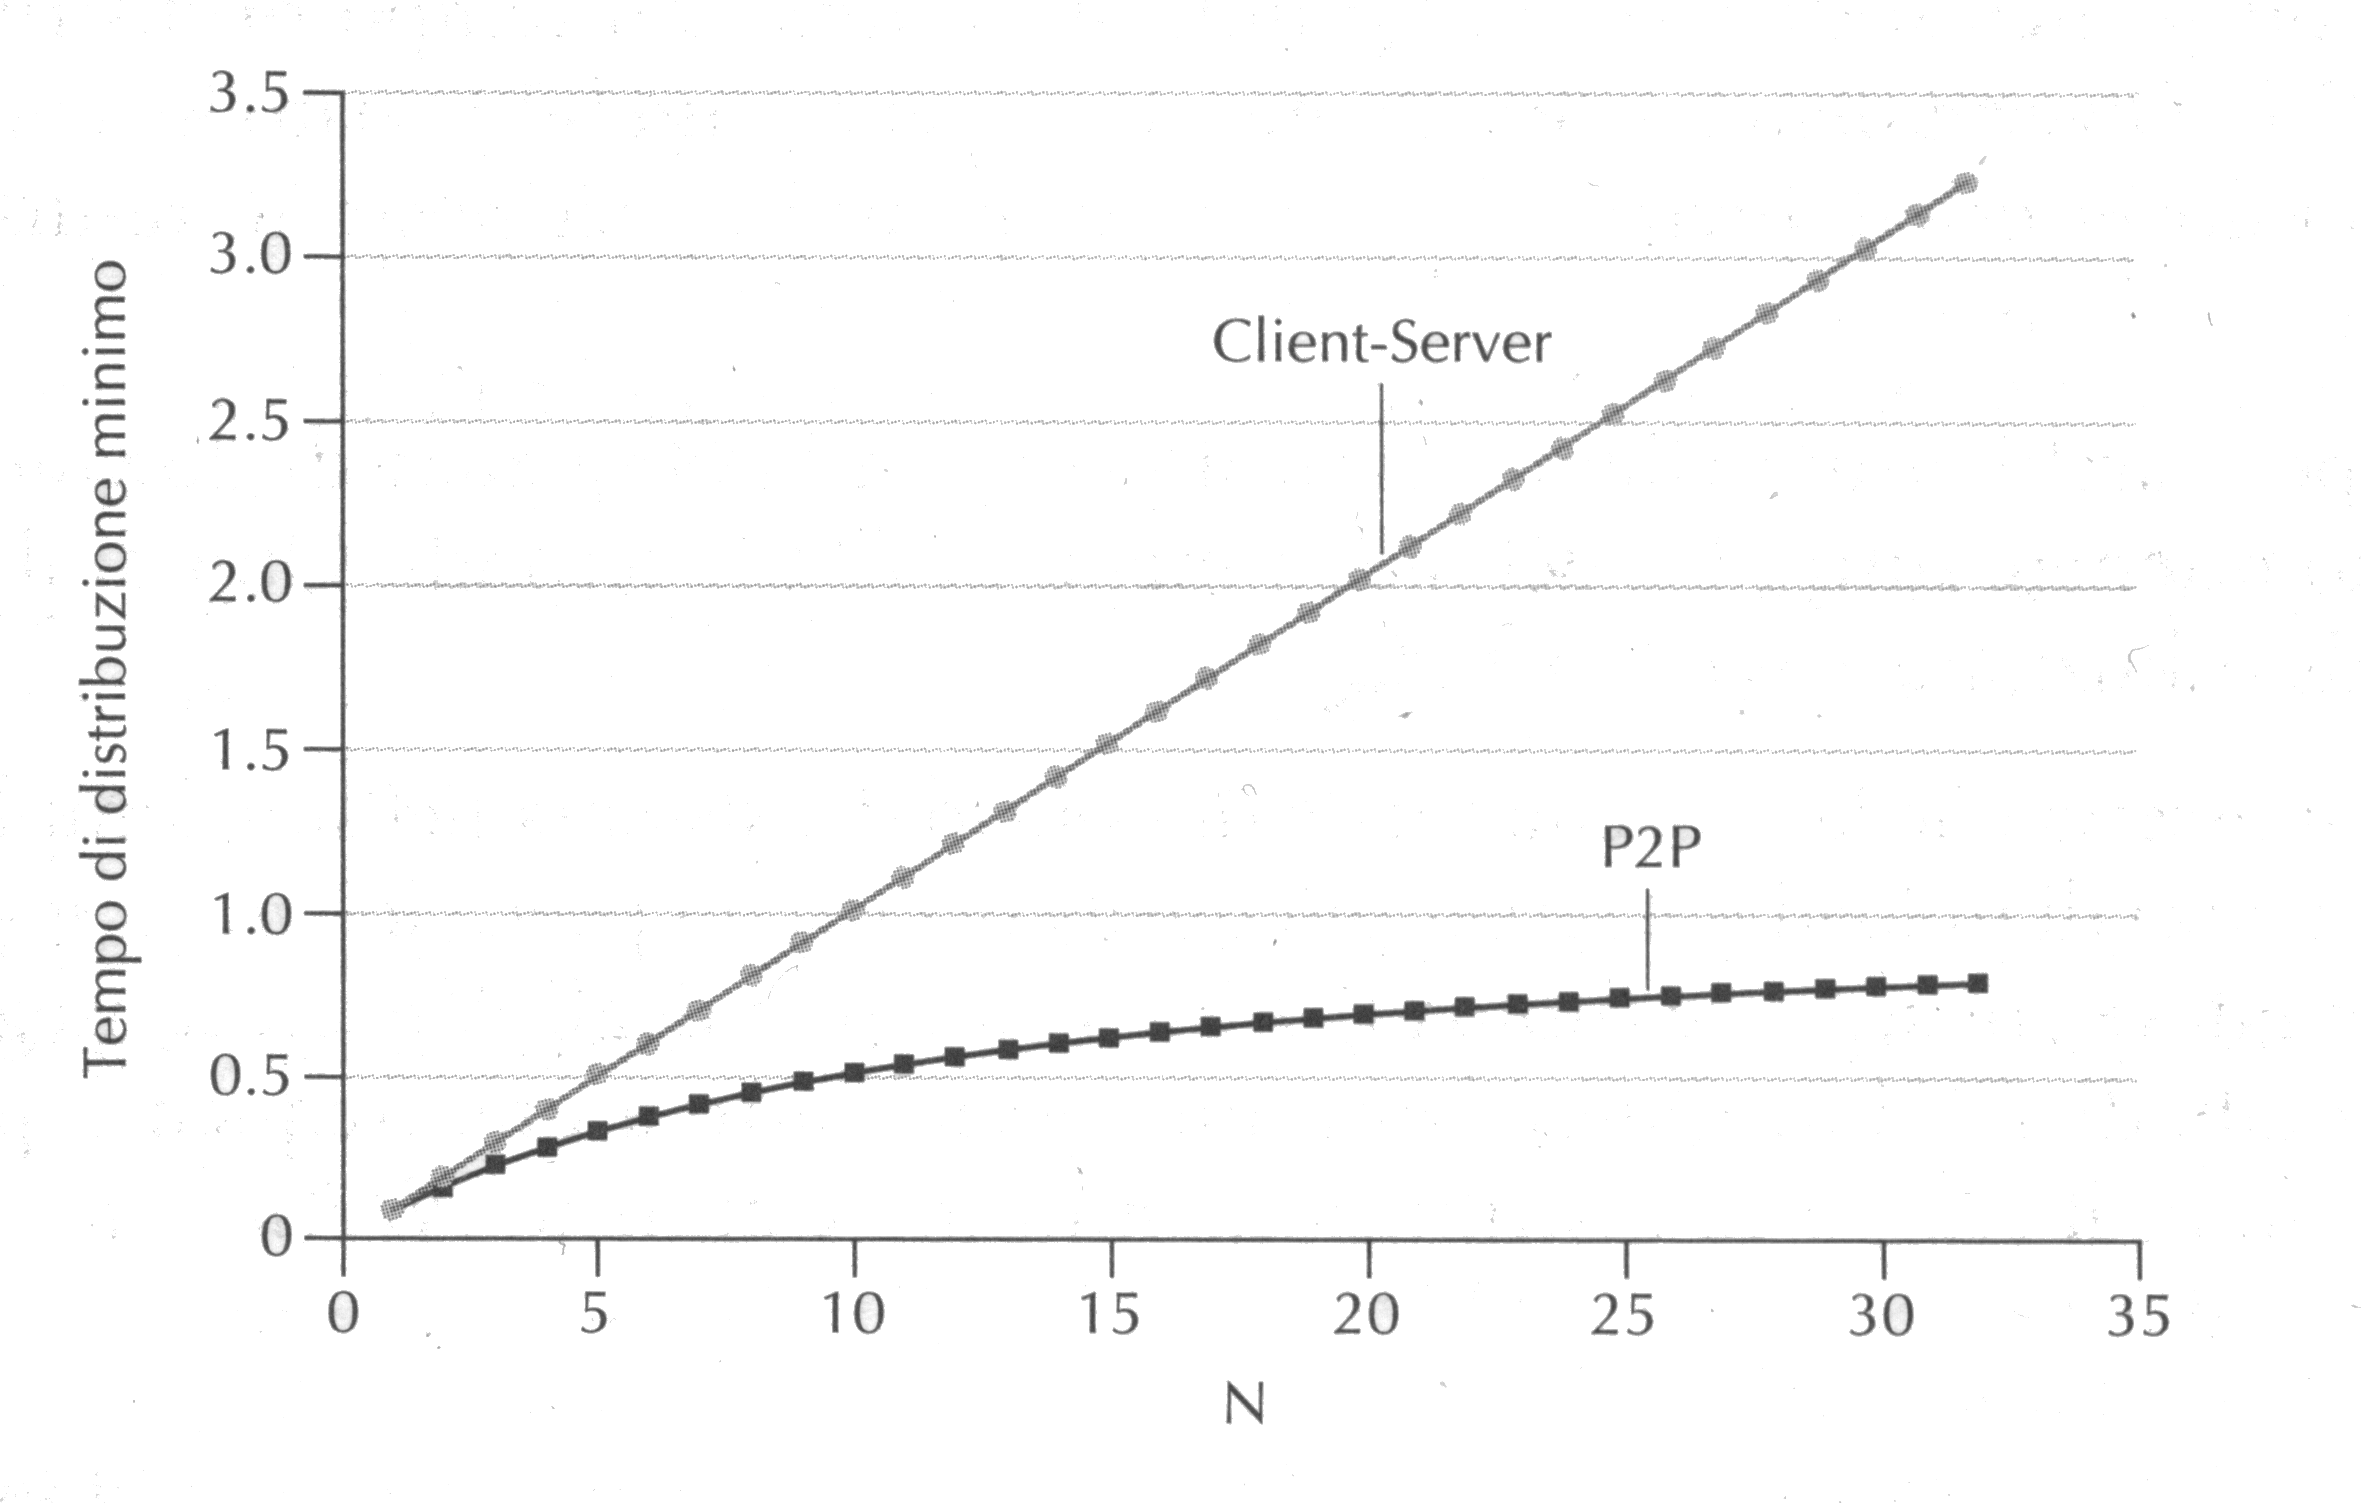
\includegraphics[scale=1]{kurose.png}
\caption[Tempi di distribuzione]{Tempi di distribuzione a confronto per le architetture P2P e client-server.\label{img_kurose}}
\end{figure}

Si nota subito che per l'architettura client-server il tempo di distribuzione risulta essere lineare come calcolato, ma ancora più notevole è il tempo di distribuzione per l'architettura P2P che non solo è sempre minore della controparte client-server, ma addirittura risulta quasi costante all'aumentare del numero dei peer. Questo dimostra come le reti P2P siano estremamente scalabili, e non c'è da stupirsi come il successo di una particolare rete dipenda essenzialmente dal numero di peer presenti. %FIXME: questa è detta molto male.

\subsection{Ricerca di informazioni}\label{ricerca-di-informazioni}

Si è parlato all'inizio della sezione di come i peer siano consapevoli di cosa altri peer stanno scaricando. Questo sottointende che esiste un sistema all'interno della rete per stabilire quanti peer sono connessi e cosa stanno condividendo e/o scaricando. Ciò significa che tale meccanismo si deve attivare ogniqualvolta un peer si (dis)connette (d)alla rete e un file viene rimosso/aggiunto. L'operazione di aggiunta/rimozione dinamica di un peer/file prende il nome di \textbf{churn}. Vediamo quindi come è possibile ricercare informazioni all'interno di una rete P2P quindi, nello specifico del file-sharing, e come sia possibile per un peer sapere quali file sono a disposizione presso quali altri peer.

\subsubsection{Directory centralizzata}\label{directory-centralizzata}

La prima, grande applicazione P2P commercializzata (\emph{Napster}) faceva uso di un indice centralizzato localizzato su un potente sever centrale. Quando un utente si collegava alla rete, l'applicazione Napster informava tale server dell'indirizzo IP della macchina e del nome dei file che l'utente aveva scelto di condividere con la rete. Il server raccoglieva quindi queste informazioni da tutti i peer collegati e aggiornava il proprio indice collegando ciascun nome di file agli indirizzi IP dei peer che in quel momento lo stavano condividendo. Ovviamente alla disconnessione di un peer l'indice veniva aggiornato di conseguenza.

Si noti come questa fosse di fatto un'architettura ibrida: client-server nella ricerca dei contenuti, P2P nel trasferimento degli stessi.

La semplicità di questo metodo nasconde però alcuni gravi difetti. Il server dell'indice si trova infatti ad essere l'anello debole della rete: un suo guasto ha come conseguenza il crollo dell'intera rete, impedendo di fatto le ricerche. Inoltre tale server deve potenzialmente gestire milioni di utenti contemporaneamete (in quanto si è visto che la potenza delle reti P2P sta nel numero di peer) e quindi risulta essere estremamente costoso da installare e mantenere, oltre a rappresentare un potenziale collo di bottiglia per l'intera rete (Napster era infatti nota per i gravi problemi di traffico da cui era afflitta).

Esiste inoltre un terzo problema non strettamente tecnico ma fondamentale per l'argomento di questo documento: \textbf{la privacy dell'utente}. Con un indice centrale che associa un file ad una serie di IP, è facile per chiunque vedere chi possiede cosa, soprattuto nel caso in cui i file condivisi rappresentino una violazione del diritto d'autore. Pur essendo il caricamento dei file una responsabilità dei singoli utenti e non di chi fornisce il servizio, molte legislazioni internazionali prevedono leggi per la tutela del copyright che possono costringere il proprietario del server ad interrompere il servizio, bloccando così l'intera rete, anche quei peer che condividevano materiale lecito. Questo controllo a volte molto invasivo (se non dannoso) da parte di terze parti non coinvolte nella rete è uno dei motivi che ha portato alla nascita di reti sempre più decentralizzate, come appunto la rete Bitcoin.

\subsubsection{Query flooding}\label{query-flooding}
 Rimanendo nell'ambito della ricerca di informazioni per file-sharing, la soluzione diametralmente opposta alla precedente risiede nell'approccio completamente distribuito del query flooding, implementato originariamente dal protocollo \textbf{Gnutella}. Questo approccio prevede che l'indice sia distribuito all'interno della comunità, in particolare ogni peer indicizza solamente quello che intende condividere con gli altri peer.

Il protocollo Gnutella prevede che ogni peer sia collegato al massimo a dieci altri nodi dell'overlay network, nodi che vengono denominati \emph{vicinato}. Se un peer vuole cercare un file, invia messaggi di ricerca ai suoi vicini, i quali instradano tali messaggi ai loro vicini che ripetono l'operazione e così via. Questo è il processo del \emph{query flooding} in cui la rete viene ``sommersa'' (\emph{flood}) di richieste (\emph{query}). Quando un peer riceve una query, controlla se nel suo indice è presente una qualche corrispondenza e, in caso affermativo, invia al peer che ha effettuato la richiesta un messaggio di successo (\emph{query-hit}) contenente il nome del file e la dimensione. La query-hit viene inviata al nodo che ha effettuato la ricerca seguendo lo stesso percorso seguito dal pacchetto query. Dopo qualche tempo il peer di origine avrà un elenco di peer che condividono file corrispondenti alla sua richiesta.

Ma anche in questo approccio, la semplicità nasconde alcune problematiche. La più grave riguarda le ricerche, che vengono propagate all'intera rete di copertura generando una enorme quantità di traffico nella rete sottostante (nel caso di Gnutella, Internet) che connette i peer. Come soluzione a tale problema si è inserito nei messaggi di ricerca di Gnutella un campo \emph{time-to-live}, il quale viene decrementato da ogni peer prima di reinoltrare la richiesta: quando il campo arriva a 0 la richiesta non viene più inoltrata, limitando quindi il raggio di azione della query. Tuttavia in questo modo si riduce anche il numero di peer contattati e la probabilità di ricevere una query-hit.

Esiste inoltre una difficoltà intrinseca alle reti P2P che Napster aveva evitato: il churn. Il protocollo Gnutella tenta di risolvere il problema in questo modo:

\begin{enumerate}
\def\labelenumi{\arabic{enumi}.}
\item
  Per prima cosa, un peer, chiamiamolo X, che vuole connettersi alla   rete deve conoscere almeno un altro peer che è già connesso alla rete   (\textbf{problema del bootstrap}). I due approcci più comuni   consistono nel mantenere in ogni peer una lista di client noti a cui   tentare di connettersi e/o, in mancanza di connessione a tali nodi,   nello scaricare una lista di nodi attualmente online da un sito
  \emph{tracker}.
\item
  Dopo aver ottenuto i nodi di bootstrap, X deve tentare di connettersi   ad ognuno di questi nodi, fino a riuscirci con uno che chiameremo Y.
\item
  Dopo la connessione, X invia ad Y un messaggio di \emph{ping}   contenente un campo contatore di peer. Y inoltra tale messaggio a   tutte i nodi nella sua rete di copertura, i quali continuano l'inoltro   fino a quando il contatore non si azzera.
\item
  Ogni volta che un peer Z riceve il \emph{ping}, risponde inviando un   messaggio \emph{pong} contenente il proprio IP attraverso la rete di   copertura fino ad X.
\item
  Grazie ai messaggi \emph{pong}, X viene a conoscenza di moltri altri   peer online (quanti dipende dal contatore impostato nel messaggio   \emph{ping}) e può tentare di connettersi ad essi per ampliare il suo   vicinato.
\end{enumerate}

\subsubsection{Copertura gerarchica}\label{copertura-gerarchica}

Avendo descritto gli approcci diametralmente opposti, vediamo ora la proverbiale via di mezzo, il modello di copertura gerarchica. L'obiettivo è ottenere il meglio dalle due implementazioni sopra descritte, e fu per la prima volta realizzato da FastTrack, un protocollo implementato in Kazaa e Morpheus. Una variante di questo modello è tutt'oggi utilizzata dall'evoluzione di Gnutella, Gnutella2. Come per il query flooding, anche questo è un modello decentralizzato, ma a differenza di esso (e a discapito del principio Peer-to-Peer) non tutti i peer sono uguali: come il nome fa suggerire, esiste una gerarchia di peer che assegna a quelli più potenti (leggasi, quelli con più banda) alcune responsabilità in più designandoli come leader per altri peer. Ogni nuovo peer deve stabilire una connessione con un leader a cui notifica tutti i file che intende condividere, creando quindi una sorta di mini indice centralizzato rispettavamente ai peer connessi a quel leader (solitamente nell'ordine del centinaio). A differenza del modello centralizzato però, i leader non sono server dedicati, bensì peer veri e propri in collegamento tra di loro. Il risultato è che i leader sono collegati ad una rete di copertura del tutto simile a quella del modello query flooding, modello utilizzato infatti per l'inoltro delle ricerche. La ricerca di un file da parte di un peer segue quindi due fasi: una richiesta al proprio leader che provvede a consultare il suo indice e una eventuale propagazione della richiesta tramite query flooding da parte del leader agli altri leader. Questa struttura ``a strati'' permette quindi la connessione di molti peer senza generare una quantità eccessiva di traffico nella rete ``ospite''.

\subsubsection{DHT (Distributed Hash Table)}\label{dht-distributed-hash-table}

Crea un indice completamente distribuito che fa corrispondere gli identificatori dei file alla loro posizione. Consente agli utenti di determinare tutte le posizioni di un file senza generare un'eccessiva quantità di traffico di ricerca. Overnet (Kademlia) sfrutta DHT come anche BitTorrent.\\
Esistono numerose implementazione di DHT, ma esulando tutte dall'ambito di questa trattazione si invita per approfondimento a consultare \cite{distributed-computing}.
